% This is a thesis template that attempts to conform to the guidelines
% published by UTRGV's Graduate School office.

% Please report any issues to
% https://github.com/UTRGV-SMSS/Thesis-Template/issues

% The author of this template is Guillermo Garza.
% Modified by Moises Castillo to conform to June 2018 updates.


% Switch this line to the final option when submitting your thesis.
% This will correct counts and remove labels that are shown during draft mode
%\documentclass[masters,draft]{UTRGVthesis}
\documentclass[masters,final]{UTRGVthesis}
%\documentclass[masters,final, nodedication, noacknowledgments]{UTRGVthesis}
%\usepackage{mathpazo}

% set font
\setmainfont{Times New Roman}
%\setmainfont{Comic Sans MS}

% Load your packages below.
% Make hyperref and showkeys come at the end of your loaded packages
% to make sure they are not over-written.  They redefine many
% standard LaTeX commands
\usepackage{docmute} % for inputting complete documents. Useful for LyX users
\usepackage{booktabs} % for better tables
\usepackage{microtype} % for better typography
\usepackage[colorlinks=false]{hyperref}  % for urls
\usepackage{showkeys} % shows labels during draft mode
%\usepackage[document]{ragged2e} % uncomment for non-justified text


% Uncomment the line below to check if text is aligned to margins
%\margins

% To change body font from Times Roman to Times New Roman, compile with XeLaTeX
% This assumes you have Times New Roman font installed in your machine
% WARNING! This will NOT change the font in Math Environments
\usepackage{ifxetex}
\ifxetex{}
   \usepackage{fontspec}
   \setmainfont{Times New Roman}
\fi


% this sets the name of the bibliography
% add \vspace{1cm} here to adjust vertical spacing after bibliography title
\renewcommand{\bibname}{BIBLIOGRAPHY}


% Insert your name and major here in the format shown
\Author{Moises Castillo}
\AuthorLastFirst{Castillo, Moises}
\Major{Physics}


% Insert your graduation date here
\Month{August}
\Year{2019}


% Insert the title of your thesis here.
% If you have a long title, split it between multiple lines using the \\ command
% Also, use comment characters to avoid unwanted spaces in the Abstract page
\Title{Pipeline for variable star detection and\\
eclipsing binary classification}


% Insert your research advisor and his title here
\Advisor{Dr.\ Mario Diaz}
\AdvisorTitle{Chair of Committee}


% Insert the members of your committee here
% You can also give MemberA a special title
\MemberA{Dr.\ Member A}  %\MemberATitle{Co-Chair of Committee}
\MemberB{Dr.\ Member B}
\MemberC{}
\MemberD{}
\MemberE{}


% Insert the text of your abstract below.
% The bibliography style "citation" required by the manual is automatically
% generated.  Specify the "final" option in the \documentclass to update the
% counts to the correct values.
\Abstract{%
    An abstract is a brief summary often used to help the reader quickly
    ascertain the paper's purpose. To be written at the end. $12345$
}


% You can dedicate your paper here.  This is optional.
\Dedication{%
    Dedication should be simple, in good taste, and fit on one page.
}


% Acknowledge those who helped and supported you here. This is optional.
\Acknowledgments{%
    Acknowledgements should be simple, in good taste, and fit on one page. CTMO, CGWA
}


% Insert your biographical sketch here.
\BiographicalSketch{%
    A brief biographical sketch of the student is required as part of each thesis.
}



\begin{document}

% This starts page counting in Roman numerals
\frontmatter


% This command makes the formal preliminary pages.
% You can comment it out during the drafting process if you want to save paper.
\makepreliminarypages{}

% These insert a table of contents, list of tables, and list of figures
\tableofcontents
\listoftables
\listoffigures


% This starts regular page counting in Arabic numerals
\mainmatter{}

% This starts double-spaced text.  Opposite command is \singlespacing
\doublespacing{}


% OK. Everything is set up. Insert your thesis below.
% It's a good idea to split your thesis up into different files and use
% the \input command
\chapter{Introduction}
\label{ch:intro}

\section{Variable stars}
Stars are called variable when there is a detectable change in brightness or color on time scales of the order
of the mean life time of humans~\cite{percy_2007, sterken_1996}.
The first claimed documented variable star is Algol visible with the unaided eye.
There exists ancient Egyptian calendars of lucky and unlucky days that possibly contain the periodicity of Algol\cite{porceddu_2008, porceddu_2018}.
The Cairo Calendar dated to 1244--1163 BC has been shown by Porceddu et al.~\cite{porceddu_2015} to represent Algol as Horus, a sky god and
symbol of kingship,
as seen in the figure~\ref{fig:horus} by matching the actions of Horus and the events witnessed by an observer of Algol.

\begin{figure}[h]
    \centering
    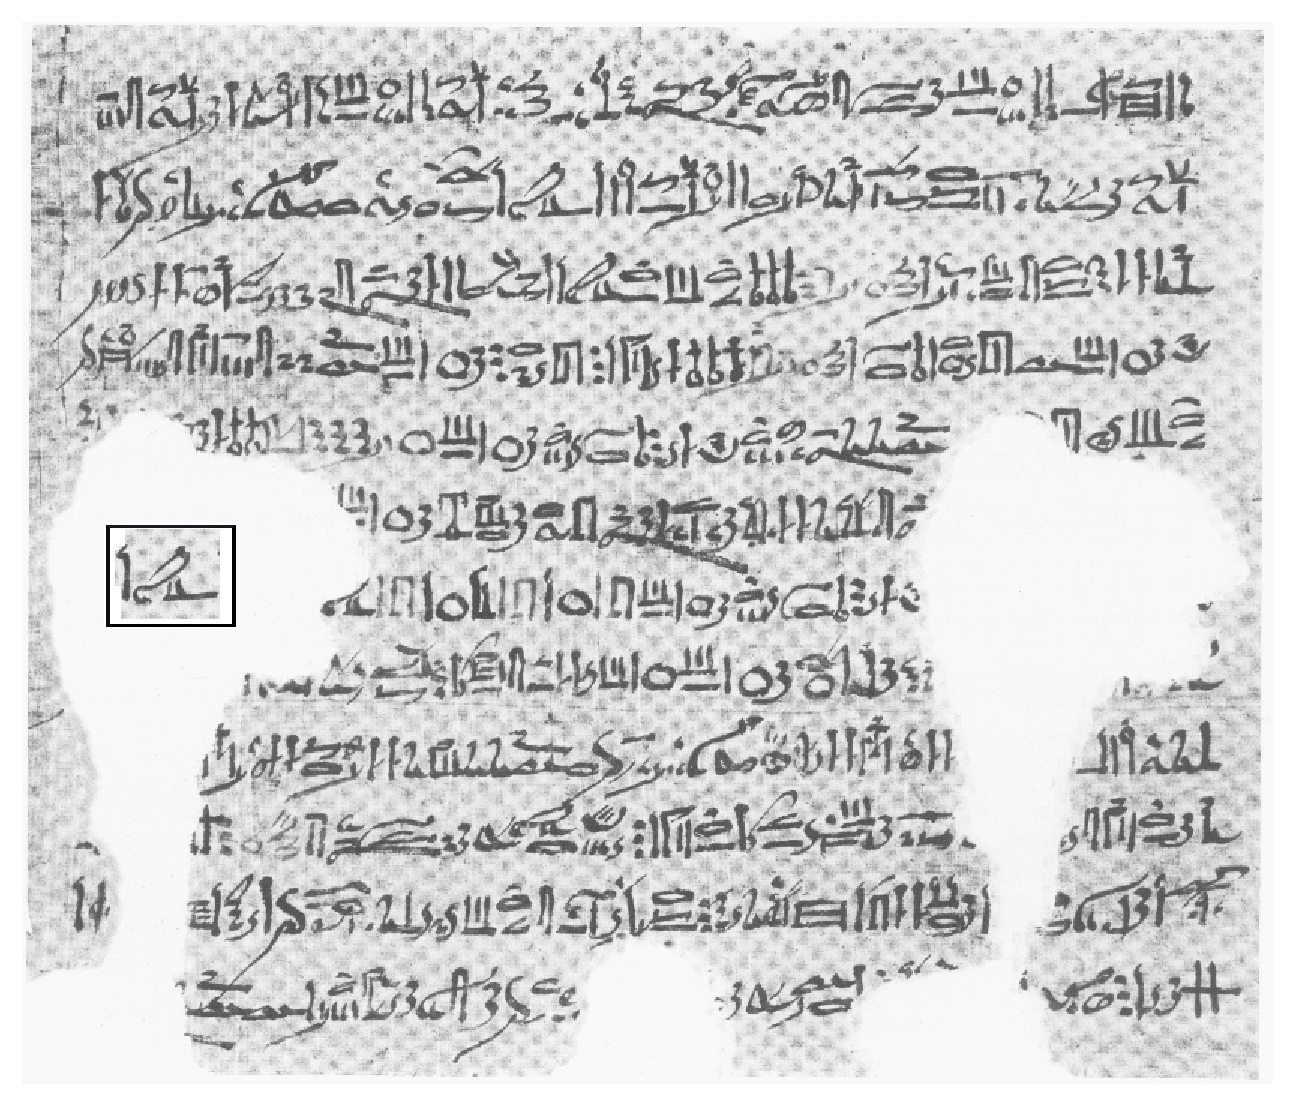
\includegraphics[width=\columnwidth]{figures/horus.eps}
    \caption{Inside the rectangle is the hieratic writing for the word Horus~\protect\cite{porceddu_2015}.}
\label{fig:horus}
\end{figure}

There is some curious relation between ancient Greek stories of the Gorgon Medusa, Perseus, the corresponding constellations, 
and the variable stars Algol and Omicron Ceti or more commonly named Mira (the wonderful).
Wilk~\cite{wilk_1996} suggests that the variability and location in the sky is embedded within the stories themselves.

The first recognized documented variable star, Omicron Ceti,  was recorded in 1596 and again in 1609 by David Fabricius while observing Jupiter.
Fabricius had first recorded Omicron Ceti as a nova, a singular event observed as a bright flash and quick dimming over the next few days,
comparing its significance with a supernova recorded by Tycho Brahe in 1572.
In 1638, Omicron Ceti was rediscovered by Johannes Phocylides Holwarda who found the periodic nature of this star to be approximately 11 months~\cite{hockey_2007}.

%In order to characterize eclipsing binary systems a light curve must be made.
%A light curve is a time series plot of the measured magnitude.

\section{Classifying variability}
Over time there have been several attempts to classify variable stars.
Classification systems reflect the current understanding of the mechanisms behind variability.
The earliest variable star observers like Goodricke and Pigott, who was employed to verify the variability of stars~\cite{pigott_1785}, would try to make sense of the observations and periods recorded by comparing and grouping different stars to those like Algol and $\omicron$ Ceti.  

One of the first attempts that went into detail was made by E.\ C.\ Pickering~\cite{sterken_1996, hoffleit_1972} in 1881 where he classified variable stars into the following categories\cite{pickering_1881}:
\begin{description}
    \item [Type I] Temporary stars. Examples, Tycho Brahe's star of 1572, new star in Corona, 1866.
    \item [Type II] Stars undergoing great variations in light in periods of several months or years. Examples, $\omicron$ Ceti and $\chi$ Cygni.
    \item [Type III] Stars undergoing slight changes according to laws yet unknown
    \item [Type IV] Stars whose light is continually varying, but the changes are repeated with great regularity in a period not exceeding a few days. 
    \item [Type V] Stars which every few days undergo for a few hours a remarkable diminution in light, this phenomenon recurring with great regularity. 
\end{description}

As time passes with more observations of variable stars, the collective understanding of the mechanisms of variability are improved.
With an improved understanding of physical processes including stellar evolution, pulsation, rotation, and eclipsing, then the taxonomy of classes is refined.

Since 1946, on behalf of the International Astronomical Union (IAU), Moscow variable star researchers have compiled detailed catalogs and certified 
variable stars in the General Catalogue of Variable Stars (GCVS). 
GCVS 5.1 is the most current version of the catalog containing $52,011$ variable objects discovered and named as variable stars by 2015~\cite{samus_2017}.

\subsection{General Catalogue of Variable Stars 5.1 Variability Types}
Variability types are in groups according to the major astrophysical reasons for variability.
The variable types have letter designations that typically corresponds to the original star that is observed with the same type of variability.
For example, in the eruptive group there is a type called GCAS that signifies eruptive irregular variables of the Gamma Cas type.
The definitions of the variable types are given by GVCS and maintained on their
website: \url{http://www.sai.msu.su/gcvs/gcvs/}

The following are groups with the variable types in those groups.
The reader can visit the GCVS Variability Types webpage\footnote{GCVS Variability Types: \url{http://www.sai.msu.su/gcvs/gcvs/vartype.htm}} to 
see specific variable types. 
\begin{description}
    \item [eruptive] FU, GCAS, I, IA, IB, IN, INA, INB, INT, IT, IN (YY), IS, ISA, ISB, RCB, RS, SDOR, UV, UVN, WR,
    \item [pulsating] ACYG, BCEP, BCEPS, CEP, CEP (B), CW, CWA, CWB, DCEP, DCEPS, DSCT, DSCTC, GDOR, L, LB, LC, M, PVTEL, RPHS, RR, RR (B), RRAB,
           RRC, RV, RVA, RVB, SR, SRA, SRB, SRC, SRD, SXPHE, ZZ, ZZA, ZZB,
    \item [rotating] ACV, ACVO, BY, ELL, FKCOM, PSR, SXARI,
    \item [cataclysmic (explosive and novalike) variables] N, NA, NB, NC, NL, NR, SN, SNI, SNII, UG, UGSS, UGSU, UGZ, ZAND,
    \item [eclipsing binary systems] E, EA, EB, EW, GS, PN, RS, WD, WR, AR, D, DM, DS, DW, K, KE, KW, SD,
    \item [intense variable X-ray sources] X, XB, XF, XI, XJ, XND, XNG, XP, XPR, XPRM, XM,
    \item [other symbols] BLLAC, CST, GAL, L:, QSO, S, *, +, $\colon$
    \item [the new variability types] ZZO, AM, R, BE, LBV, BLBOO, EP, SRS, LPB
\end{description}

This document will not cover all the different variable stars types. 
The study specifically will focus on EW type eclipsing binary systems.  

%%%% CONSIDER OMISSION 
%% \section{Characterizing variability}
%% Using different algorithms one can distinguish the difference between the types of variable star system.
%% 
%% This demonstrates RR Lyrae
%% This demonstrates Eclipsing binaries
%% 
%% The relation between orbital mechanics and light curves
%% 
%% This demonstrates solar spots
%% 
%% Complex systems can involve a combination of these different systems.



% This makes the bibliography.
% Enter your references in the BibTex file "references.bib"
% You can find bibtex info from Google Scholar.
\bibliographystyle{siam}
\bibliography{msthesisref}


% Uncomment the \appendix macro below for appendices
% Insert appendix chapters after the macro
%\appendix


% This inserts your Biographical Sketch
\biographypage{}

\end{document}
